%\documentclass[a4paper,twocolumn]{article} % Document type

\documentclass[a4paper,12pt,oneside,onecolumn]{article} % Document type

\usepackage[left=1.0in, right=1.0in, top=1.0in, bottom=1.0in]{geometry}

\ifx\pdfoutput\undefined
    %Use old Latex if PDFLatex does not work
   \usepackage[dvips]{graphicx}% To get graphics working
   \DeclareGraphicsExtensions{.eps} % Encapsulated PostScript
 \else
    %Use PDFLatex
   \usepackage[pdftex]{graphicx}% To get graphics working
   \DeclareGraphicsExtensions{.pdf,.jpg,.png,.mps} % Portable Document Format, Joint Photographic Experts Group, Portable Network Graphics, MetaPost
   \pdfcompresslevel=9
\fi

\usepackage{amsmath,amssymb}   % Contains mathematical symbols
\usepackage[ansinew]{inputenc} % Input encoding, identical to Windows 1252
\usepackage{tikz}
\usepackage[english]{babel}    % Language
\usepackage[square,numbers]{natbib}     %Nice numbered citations
\bibliographystyle{plainnat}            %Sorted bibliography



\begin{document}               % Begins the document

\title{Homework 3 (Tasks 1-19) in EL2450 Hybrid and Embedded Control Systems}
\author{
  Rene Garcia \\ 20010124-5512 \\ reneogt@kth.se
  \and
  Daniel Skott \\ 20020314-5214 \\ dskott@kth.se
  \and
  Joel Aggefors \\ 20030301-4575 \\ joelag@kth.se
  \and
  Jenis Jain \\ 20030424-T490 \\ jjjain@kth.se
  \and
  David Ring \\ 20000111-2374 \\ dring@kth.se
  \and
  }
%\date{2010-10-10}             % If you want to set the date yourself.

\maketitle                     % Generates the title



\section*{Task 1: Compute $u_r$ and $u_l$ from $(v,\omega)$}

The robot inputs are defined as:
\begin{equation}
v = \frac{u_r + u_l}{2}, 
\qquad 
\omega = u_r - u_l .
\label{eq:vomega_def}
\end{equation}

From \eqref{eq:vomega_def}, multiply the first equation by $2$:
\begin{equation}
2v = u_r + u_l .
\label{eq:sum}
\end{equation}

Now add \eqref{eq:sum} and the second equation in \eqref{eq:vomega_def}:
\begin{equation}
2v + \omega = (u_r+u_l) + (u_r-u_l) = 2u_r
\;\;\Rightarrow\;\;
u_r = v + \frac{\omega}{2}.
\label{eq:ur}
\end{equation}

Similarly, subtract the second equation in \eqref{eq:vomega_def} from \eqref{eq:sum}:
\begin{equation}
2v - \omega = (u_r+u_l) - (u_r-u_l) = 2u_l
\;\;\Rightarrow\;\;
u_l = v - \frac{\omega}{2}.
\label{eq:ul}
\end{equation}

Therefore, the wheel speeds corresponding to $(v,\omega)$ are:
\begin{equation}
\boxed{
u_r = v + \frac{\omega}{2},
\qquad
u_l = v - \frac{\omega}{2}
}
\label{eq:wheel_from_vomega}
\end{equation}


\section*{Task 2}
% Requires: \usepackage{tikz}
% Optional: \usetikzlibrary{positioning}

\begin{figure}[h!]
\centering
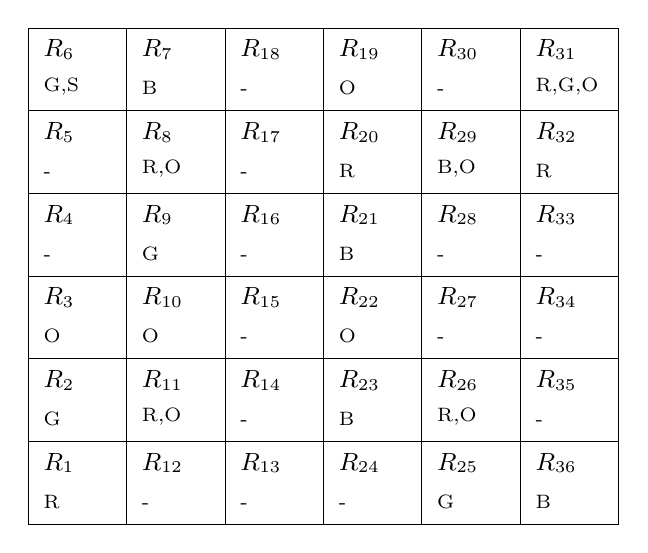
\begin{tikzpicture}[font=\small]

% --- grid settings ---
\def\w{1.25}  % cell width
\def\h{1.05}  % cell height

% Helper: draw one cell: (col,row from top-left), region label, AP text
\newcommand{\cell}[4]{%
  \draw (#1*\w, -#2*\h) rectangle ++(\w,\h);
  \node[anchor=north west] at (#1*\w+0.07, -#2*\h+0.98*\h) {$#3$};
  \node[anchor=south west, font=\scriptsize] at (#1*\w+0.07, -#2*\h+0.08) {#4};
}

% Row 1 (top)
\cell{0}{0}{R_6}{G,S}
\cell{1}{0}{R_7}{B}
\cell{2}{0}{R_{18}}{-}
\cell{3}{0}{R_{19}}{O}
\cell{4}{0}{R_{30}}{-}
\cell{5}{0}{R_{31}}{R,G,O}

% Row 2
\cell{0}{1}{R_5}{-}
\cell{1}{1}{R_8}{R,O}
\cell{2}{1}{R_{17}}{-}
\cell{3}{1}{R_{20}}{R}
\cell{4}{1}{R_{29}}{B,O}
\cell{5}{1}{R_{32}}{R}

% Row 3
\cell{0}{2}{R_4}{-}
\cell{1}{2}{R_9}{G}
\cell{2}{2}{R_{16}}{-}
\cell{3}{2}{R_{21}}{B}
\cell{4}{2}{R_{28}}{-}
\cell{5}{2}{R_{33}}{-}

% Row 4
\cell{0}{3}{R_3}{O}
\cell{1}{3}{R_{10}}{O}
\cell{2}{3}{R_{15}}{-}
\cell{3}{3}{R_{22}}{O}
\cell{4}{3}{R_{27}}{-}
\cell{5}{3}{R_{34}}{-}

% Row 5
\cell{0}{4}{R_2}{G}
\cell{1}{4}{R_{11}}{R,O}
\cell{2}{4}{R_{14}}{-}
\cell{3}{4}{R_{23}}{B}
\cell{4}{4}{R_{26}}{R,O}
\cell{5}{4}{R_{35}}{-}

% Row 6 (bottom)
\cell{0}{5}{R_1}{R}
\cell{1}{5}{R_{12}}{-}
\cell{2}{5}{R_{13}}{-}
\cell{3}{5}{R_{24}}{-}
\cell{4}{5}{R_{25}}{G}
\cell{5}{5}{R_{36}}{B}

\end{tikzpicture}
\caption{Workspace discretization with $K=36$ regions. Labels indicate where atomic propositions hold.}
\label{fig:gridK36}
\end{figure}



\subsection*{(a) Discretization, numbering , and atomic propositions}

\textbf{Workspace:} $[-1.5,1.5]\times[-1.5,1.5]$ (meters). A discretization with $K=36$ gives a $6\times 6$ grid.

The regions are numbered in a \emph{column-wise snake} pattern:
start at the bottom-left with $R_1$, go \emph{up} in the first column, then \emph{down} in the next column, and so on.
Thus, the $6\times 6$ numbering is:
\[
\begin{array}{|c|c|c|c|c|c|}
\hline
R_{6} & R_{7} & R_{18} & R_{19} & R_{30} & R_{31}\\ \hline
R_{5} & R_{8} & R_{17} & R_{20} & R_{29} & R_{32}\\ \hline
R_{4} & R_{9} & R_{16} & R_{21} & R_{28} & R_{33}\\ \hline
R_{3} & R_{10} & R_{15} & R_{22} & R_{27} & R_{34}\\ \hline
R_{2} & R_{11} & R_{14} & R_{23} & R_{26} & R_{35}\\ \hline
R_{1} & R_{12} & R_{13} & R_{24} & R_{25} & R_{36}\\
\hline
\end{array}
\]

\textbf{Atomic propositions:}
Let $AP=\{\textsf{red},\textsf{blue},\textsf{green},\textsf{obstacle}\}$.
The propositions are specified by the following positions (meters):

\begin{itemize}
\item \textsf{obstacle} centers (spheres of radius $0.05$ m) at:
\[
\begin{aligned}
(-0.75,0.75),\ (0.25,1.25),\ (0.75,0.75),\ (0.25,-0.25),\ (0.75,-0.75),\ (-0.75,-0.75),\\
(-0.75,-0.25),\ (1.25,1.25),\ (-1.25,-0.25).
\end{aligned}
\]
\item \textsf{red} holds at:
\[
(-0.75,0.7),\ (0.2,0.7),\ (1.25,1.25),\ (1.2,0.8),\ (0.8,-0.8),\ (-0.9,-0.8),\ (-1.25,-1.25).
\]
\item \textsf{blue} holds at:
\[
(-0.75,1.4),\ (0.9,0.9),\ (0.3,0.2),\ (0.25,-0.75),\ (1.2,-1.4).
\]
\item \textsf{green} holds at:
\[
(-1.23,1.25),\ (1.25,1.25),\ (-0.9,0.2),\ (-1.2,-0.7),\ (0.6,-1.2).
\]
\end{itemize}

\textbf{Labeling rule:} a proposition is true in the region that contains its given position, i.e.
\[
p\in L(R_i)\ \Longleftrightarrow\ (x_p,y_p)\in R_i,\qquad p\in AP.
\]
The start position is $(-1.25,1.25)$, hence $S_0=\{R_6\}$.

\subsection*{(b) Cell size $dx,dy$}
Since the side length is $3$ m and there are $6$ cells per side,
\[
dx=\frac{3}{6}=0.5\ \text{m},\qquad dy=\frac{3}{6}=0.5\ \text{m}.
\]

\subsection*{(c) Comment on the choice $K=36$}
A $6\times 6$ grid provides a finer abstraction than coarse grids (better separation of obstacles/colored areas),
but increases the number of states and transitions compared to smaller $K$.

\subsection*{(d) Transition system $T=(S,S_0,\Sigma,\rightarrow,AP,L)$}
\[
S=\{R_1,\dots,R_{36}\},\qquad S_0=\{R_6\},\qquad
\Sigma=\{\textsf{Up},\textsf{Down},\textsf{Left},\textsf{Right}\},\qquad
\newline AP=\{\textsf{red},\textsf{blue},\textsf{green},\textsf{obstacle}\}.
\]
The transition relation $\rightarrow$ is the 4-neighborhood relation on the grid:
\[
R_i \xrightarrow{\sigma} R_j
\quad\Longleftrightarrow\quad
R_j \text{ is the adjacent region to } R_i \text{ in direction } \sigma\in\Sigma.
\]
The labeling function $L:S\to 2^{AP}$ is defined using the point-in-region rule above.


\section*{Task 3: Find an infinite path satisfying the specification}

\textbf{Specification:}
(i) visit \textsf{red} infinitely often,
(ii) whenever the robot is in a \textsf{red} region, the \emph{next} region is \textsf{blue},
(iii) never enter a region labeled \textsf{obstacle}.

\medskip
\textbf{Chosen \textsf{red}--\textsf{blue} pair:}
From the labeling in Task 2, $R_{20}\in \textsf{red}$ and $R_{21}\in \textsf{blue}$, and they are adjacent in the $6\times 6$ grid
($R_{21}$ is directly below $R_{20}$). Moreover, $R_{20},R_{21}\notin \textsf{obstacle}$.

\medskip
\textbf{A valid infinite path:}
Starting from $S_0=\{R_6\}$, one feasible prefix to reach $R_{20}$ without entering obstacles is
\[
R_6 \;\rightarrow\; R_7 \;\rightarrow\; R_{18} \;\rightarrow\; R_{17} \;\rightarrow\; R_{16} \;\rightarrow\; R_{21} \;\rightarrow\; R_{20}.
\]
Then, repeat the 2-cycle $(R_{20},R_{21})$ forever:
\[
\pi \;=\; \underbrace{\big(R_6, R_7, R_{18}, R_{17}, R_{16}, R_{21}, R_{20}\big)}_{\text{prefix}}
\;\cdot\;
\underbrace{\big(R_{21},R_{20}\big)^{\omega}}_{\text{suffix repeated forever}}.
\]

\medskip
\textbf{Why $\pi$ satisfies the specification:}
\begin{itemize}
\item $\pi$ visits $R_{20}$ infinitely often, and $R_{20}\in\textsf{red}$, hence \textsf{red} is visited infinitely often.
\item Every time $\pi$ is in $R_{20}$ (a \textsf{red} region), the next state is $R_{21}$ and $R_{21}\in\textsf{blue}$, so the ``after \textsf{red} next is \textsf{blue}'' condition holds.
\item All regions used in $\pi$ are chosen outside the set of \textsf{obstacle} regions, hence obstacles are never entered.
\end{itemize}

\section*{Task 4}

The hybrid strategy prevents entering unintended regions by separating the motion into two simple phases. First, the robot uses a rotation mode with (approximately) zero forward
speed, i.e., $v \approx 0$, so it turns in place to align its heading with the straight line
connecting the center of the current region to the center of the target (neighbor) region.
Because the robot does not translate during this phase, it stays close to the current
region center and does not drift into adjacent regions. Second, the robot switches to a
line-following mode and drives forward while tracking that same center-to-center line.
For neighboring regions, this line segment lies within the union of the two adjacent cells.
Therefore, if the tracking error is kept small, the robot remains inside only the current and
target regions during the transition, and it avoids passing through any other region that
could contain an obstacle.

\section*{Task 5}

During the rotation mode, the controller is
\begin{equation}
\omega[k] = K_{\Psi,1}\big(\theta_R-\theta[k]\big).
\label{eq:rot_ctrl}
\end{equation}
The robot yaw dynamics satisfy
\begin{equation}
\dot{\theta}(t) = \frac{R}{L}\,\omega(t).
\label{eq:yaw_dyn}
\end{equation}
Using forward Euler discretization with sampling time $h$,
\begin{equation}
\theta[k+1] = \theta[k] + h\frac{R}{L}\omega[k].
\label{eq:euler}
\end{equation}
Substituting \eqref{eq:rot_ctrl} into \eqref{eq:euler} and defining the error
$e[k]=\theta_R-\theta[k]$, we obtain
\begin{equation}
e[k+1] = \Big(1-\frac{hR}{L}K_{\Psi,1}\Big)e[k].
\label{eq:error_dyn}
\end{equation}
For asymptotic stability of the discrete-time error dynamics, we require
\begin{equation}
\left|1-\frac{hR}{L}K_{\Psi,1}\right|<1
\;\;\Longleftrightarrow\;\;
0<\frac{hR}{L}K_{\Psi,1}<2
\;\;\Longleftrightarrow\;\;
\boxed{\,0<K_{\Psi,1}<\frac{2L}{hR}\, }.
\label{eq:stability_range}
\end{equation}
A practical choice is to pick $K_{\Psi,1}$ well inside this interval (e.g., $K_{\Psi,1}=\alpha\frac{L}{hR}$ with $\alpha\in(0,1)$) to avoid oscillations and actuator saturation.


\section*{Task 6}
First we define the proportional constant value. Given eq. \eqref{eq:stability_range}, we could 
aim for a deadbeat controller by setting $K_{\Psi,1}=\frac{2L}{hR}$, nonetheless, this would force
the controller to correct the error in one sampling step, completely ignoring physical limits and
inertia. A safer value to chose is the middle of the stability range:
\begin{equation}
K_{\Psi,1}=\frac{1}{2}\frac{2L}{hR}=\frac{L}{hR}=\frac{0.16}{0.033*1} = 4.85\quad [1/s].
\end{equation}
To test the performance of the  controller, we run 2 different scenarios:
\begin{itemize}
\item \textbf{Scenario 1:} $\theta_R=90^\circ$, $\theta[0]=0^\circ$ (90 degree turn)
\begin{center}
  \includegraphics[width = 0.7\textwidth]{ss-err-90}
\end{center}
For this case, the wheels stop turning at around $1.85\,s$, and there is a \textbf{steady-state} error of $0.23^\circ$.
\item \textbf{Scenario 2:} $\theta_R=180^\circ$, $\theta[0]=0^\circ$ (180 degree turn)
\begin{center}
  \includegraphics[width = 0.7\textwidth]{ss-err-180}
\end{center}
For this case, there is a constant ripple that slowly rotates the robot back and forth around the target angle. This is a case of limit cycle caused by quantization.
For this case, we consider the largest error, that is, the peak of the ripple. Then, the \textbf{steady-state} error is $0.46^\circ$.
\end{itemize}
In general, can see that the controller \textbf{asymptotically stabilizes} the error in both scenarios, as we don't see divergence over time.
\section*{Task 7}

Assume $\theta[k+1]=\theta[k]=\theta$ so $v_c=\begin{bmatrix}\cos\theta & \sin\theta\end{bmatrix}^\top$ is constant and $v_c^\top v_c=1$.
Using $\dot{p}=R v v_c$ with $p=\begin{bmatrix}x&y\end{bmatrix}^\top$ and forward Euler,
\[
p[k+1]=p[k]+hR\,v[k]\,v_c
\;\Rightarrow\;
\Delta_0[k+1]=\Delta_0[k]-hR\,v[k]\,v_c.
\]
Premultiplying by $v_c^\top$ yields
\[
d_0[k+1]=v_c^\top\Delta_0[k+1]
=d_0[k]-hR\,v[k].
\]
With $v[k]=K_{\omega,1}d_0[k]$,
\[
d_0[k+1]=\big(1-hR K_{\omega,1}\big)d_0[k].
\]
Asymptotic stability requires $\left|1-hR K_{\omega,1}\right|<1$, hence
\[
\boxed{\,0<K_{\omega,1}<\dfrac{2}{hR}\, }.
\]
\section*{Task 8}
Similarly to Task 6, we select $K_{\omega,1}$ in the middle of the stability interval:
\begin{equation}
K_{\omega,1}=\frac{1}{2}\frac{2}{hR}=\frac{1}{hR}=\frac{1}{0.033*1} = 30.3\quad [\frac{1}{m\cdot s}].
\end{equation}
To test the performance of the  controller, we run 1 single scenario:
\begin{itemize}
% \item \textbf{Scenario 1: Longitudinal error}\\
% Starting position: $(x_0,y_0) = (0,0),\, \theta=0^\circ$ Target: $(x_g,y_g) = (-1,0)$
% \begin{center}
%   %\includegraphics[width = 0.8\textwidth]{task_8_ss-err_1}
% \end{center}
% \item \textbf{Scenario 2: Lateral Error}\\
% Starting position: $(x_0,y_0) = (0,0),\, \theta=0^\circ$ Target: $(x_g,y_g) = (0,-1)$
% \begin{center}
%   %\includegraphics[width = 0.8\textwidth]{ss-err-180}
% \end{center}
\item \textbf{Scenario 1: Diagonal Error}\\
Starting position: $(x_0,y_0) = (0,0),\, \theta=0^\circ$ Target: $(x_g,y_g) = (-1,1)$
\begin{center}
  \includegraphics[width = 0.8\textwidth]{task_8_ss-err_3}
\end{center}
As we can see, the robot moves only in the $x$ direction, as this is the direction it is facing initially. The controller successfully reduces the X error to zero, but the Y error remains.
\end{itemize}
\section*{Task 9}
To test both controllers together, we simulate an scenario where we have error in the position and angle, and enable both controllers.
\begin{itemize}
\item \textbf{Scenario 1:} Starting position: $(x_0,y_0) = (0,0),\,\theta=0^\circ$ Target: $(x_g,y_g) = (1,1),\,\theta^R=180^\circ $
\begin{center}
  \includegraphics[width = 0.7\textwidth]{task_9_combined_pos_angle}
\end{center}
\end{itemize}
As we can see, the angle error is corrected first, and then blocking the posiblitiy of correcting the position error. This can become a race condition.
\section*{Task 10}

Assume $\theta[k]=\theta_g$, hence $v_g=\begin{bmatrix}\cos\theta_g & \sin\theta_g\end{bmatrix}^\top$ is constant and $v_g^\top v_g=1$.
With $\dot{p}=R v v_g$ and forward Euler,
\[
p[k+1]=p[k]+hR\,v[k]\,v_g
\;\Rightarrow\;
\Delta_g[k+1]=\Delta_g[k]-hR\,v[k]\,v_g.
\]
Premultiplying by $v_g^\top$ yields
\[
d_g[k+1]=v_g^\top\Delta_g[k+1]=d_g[k]-hR\,v[k].
\]
Using $v[k]=K_{\omega,2}d_g[k]$,
\[
d_g[k+1]=\big(1-hR K_{\omega,2}\big)d_g[k].
\]
Asymptotic stability requires $\left|1-hR K_{\omega,2}\right|<1$, hence
\[
\boxed{\,0<K_{\omega,2}<\dfrac{2}{hR}\, }.
\]
A practical choice is to select $K_{\omega,2}$ well inside this interval (e.g.,
$K_{\omega,2}=\alpha\frac{1}{hR}$ with $\alpha\in(0,1)$) to ensure monotone convergence
and robustness to discretization/actuator limits.

\section*{Task 11}

The closed-loop dynamics of $d_g$ are
\[
d_g[k+1] = (1 - HRK_{\omega,2}) d_g[k].
\]
For $0 < HRK_{\omega,2} < 2$, we have $|1 - HRK_{\omega,2}| < 1$, hence
\[
\lim_{k\to\infty} d_g[k] = 0.
\]
Thus, $d_g$ is asymptotically stabilized in $0$.

However, since $\omega[k]=0$, the orientation $\theta$ remains constant and the robot moves along a fixed straight line. If the initial orientation is not aligned with the goal direction, the robot cannot correct lateral error. Therefore,
\[
[x[k],y[k]]^T \not\to [x_g,y_g]^T
\]
for arbitrary initial orientations.

In Fig.~\ref{fig:Task11.1} we can see that the robot travels in a straight line and that it comes closer to the goal. Another observation not observable in the graph is that the robot slows down and stops at the goal.

\begin{figure} [h!]
    \centering
    \includegraphics[width=0.5\linewidth]{result_from_task11_simulation.png}
    \caption{Result from discrete straight line controller}
    \label{fig:Task11.1}
\end{figure}

\section*{Task 12}

The controller for line-following (part II) is 
\[
\omega[k]=K_{\Psi,2}\,d_p[k].
\]
Assume the robot is on the line from $(x_0,y_0)$ to $(x_g,y_g)$ and $\theta$ is close to $\theta_g$ so that
\[
d_p[k]\approx p(\theta_g-\theta[k]), \qquad p>0. 
\]
Let $e[k]=\theta_g-\theta[k]$, hence $d_p[k]\approx p\,e[k]$.
From the yaw dynamics $\dot{\theta}=\frac{R}{L}\omega$ and forward Euler with sampling time $h$,
\[
\theta[k+1]=\theta[k]+h\frac{R}{L}\omega[k].
\]
Therefore,
\[
e[k+1]=\theta_g-\theta[k+1]=e[k]-h\frac{R}{L}\omega[k]
=e[k]-h\frac{R}{L}K_{\Psi,2}d_p[k]
\approx \Big(1-h\frac{R}{L}K_{\Psi,2}p\Big)e[k].
\]
Multiplying by $p$ gives the discrete-time dynamics of $d_p$:
\[
d_p[k+1]\approx \Big(1-h\frac{R}{L}K_{\Psi,2}p\Big)d_p[k].
\]
Thus $d_p[k]$ is asymptotically stabilized in $0$ iff
\[
\left|1-h\frac{R}{L}K_{\Psi,2}p\right|<1
\quad\Longleftrightarrow\quad
\boxed{\,0<K_{\Psi,2}<\frac{2L}{hRp}\, }.
\]
\paragraph{Choice of $K_{\Psi,2}$.}
Select $K_{\Psi,2}$ strictly inside the stability interval, e.g.
\[
K_{\Psi,2}=\alpha\,\frac{L}{hRp},\qquad \alpha\in(0,1),
\]
which yields the contraction factor $1-\alpha$ (monotone convergence) and keeps the
closed-loop behavior consistent when the sampling time $h$ changes.


\section*{Task 13}

If we model the corrective input using the (nonlinear) sine term, for instance
\[
d_p \approx p\,\sin(\theta_g-\theta),
\]
then \(p\) plays the role of a proportional gain. Increasing \(p\) improves the tracking accuracy of \(\theta\) to the goal \(\theta_g\). However, if \(p\) is chosen too large the closed-loop trajectory typicallyoscillates around \(\theta_g\) and cannot settle at a point. Intuitively this happens because the region of attraction (the set of initial conditions that converge to \(\theta_g\)) shrinks as \(p\) increases, so overly large gains reduce stability margins and promote sustained oscillations.


The angular controller

\begin{equation}    
\omega[k] = K_{\Psi,2} d_p[k]
\label{dp}
\end{equation}

\noindent was implemented using the exact nonlinear definition of $d_p$ from \eqref{dp}, while the translational velocity was set to $v=0$ to isolate the rotational dynamics.

The lateral deviation is defined as
\[
d_p[k] = v_{g,\perp}^T v_p[k],
\]
where
\[
v_p[k] =
\begin{bmatrix}
x[k] + p \cos\theta[k] - x_0 \\
y[k] + p \sin\theta[k] - y_0
\end{bmatrix}.
\]

Simulation results show that the robot rotates in place and $d_p[k]$ converges asymptotically to zero without steady-state error. The decay is approximately exponential, consistent with the discrete-time dynamics derived in Task 12:
\[
d_p[k+1]
=
\left(1 - \frac{hR}{L} K_{\Psi,2} p \right) d_p[k].
\]

For
\[
K_{\Psi,2} = \frac{\alpha L}{h R p}, \quad 0 < \alpha < 1,
\]
the closed-loop pole becomes $1-\alpha$, which lies inside the unit circle. Hence, the equilibrium $d_p=0$ is asymptotically stable.

The simulation confirms the theoretical stability analysis.

In fig \ref{fig:theta_over_time_task_13} we can see that the angle slowly goes from 0 degrees to 90 degrees when the goal point changes. in this simulation the new goal was 90 degrees above the robot with means that it reached the goal in the simulation.

\begin{figure} [h!]
    \centering
    \includegraphics[width=0.5\linewidth]{task13theta.png}
    \caption{theta over time task 13}
    \label{fig:theta_over_time_task_13}
\end{figure}

\smallskip

\textbf{Remark.} In particular one must not replace \(\sin(\theta_g-\theta)\) by \(\theta_g-\theta\) unless the small-angle approximation is explicitly justified.
\section*{Task 14}
From Task~12, the stability condition for the line-following controller is
\[
0<K_{\Psi,2}<\frac{2L}{hRp}.
\]
Since $p$ appears in the denominator, a larger $p$ shrinks the stability interval and reduces the maximum admissible gain $K_{\Psi,2}$. We compare two values experimentally:
\begin{itemize}
\item $p=0.5$: stability bound $K_{\Psi,2}<\frac{2\cdot0.16}{1\cdot0.033\cdot0.5}\approx19.4$. The wide stability margin allows a strong corrective input without oscillations. The measured displacement error is $y_{\text{err}}=0.1$\,m.
\item $p=1.0$: stability bound $K_{\Psi,2}<\frac{2\cdot0.16}{1\cdot0.033\cdot2}\approx4.85$. The narrow margin means the same gain $C$ pushes the system closer to the stability boundary, resulting in slower or oscillatory convergence. The measured displacement error is $y_{\text{err}}=0.5$\,m.
\end{itemize}

\begin{center}
  \includegraphics[width = 0.7\textwidth]{task_14_angle_correction}
\end{center}

As can be seen in the  plot, $p=0.5$ provides a smoother and faster convergence to the target angle $\theta_g=90^\circ$, while $p=1.0$ leads to a noticeably slower response with a larger displacement error. Therefore, \textbf{we choose $p=0.5$} because it offers a wider stability margin, better transient behavior, and a significantly smaller steady-state displacement error.

\section*{Task 15}

When both controllers are enabled, the longitudinal
error $d_g$ and the lateral error $d_p$ converge
simultaneously to zero. In contrast, when only the
translational controller is active, $d_g$ decreases while
$d_p$ remains nonzero. When only the angular controller
is enabled, $d_p$ converges but no progress toward the
goal is achieved. The combined controller therefore
achieves stable line-following behaviour.

\begin{figure}[h!]
    \centering
    \includegraphics[width=0.5\linewidth]{image.png}
    \caption{}
    \label{fig:placeholder}
\end{figure}



\section*{Task 16 : Hybrid automaton}

Define the hybrid automaton $H=(Q,X,Init,f,D,E,G,R)$.

\paragraph{Discrete states.}
\[
Q=\{q_{\text{rot}},\,q_{\text{line}}\},
\]
where $q_{\text{rot}}$ aligns the robot with the goal direction and $q_{\text{line}}$ performs line-following / go-to-goal.

\paragraph{Continuous state and initialization.}
\[
X=\begin{bmatrix}x\\y\\\theta\end{bmatrix},\qquad
Init=\Big\{(q_{\text{rot}},X)\ \big|\ X=\begin{bmatrix}x_s\\y_s\\\theta_s\end{bmatrix}\Big\}.
\]

\paragraph{Continuous dynamics (closed-loop).}
Robot kinematics:
\[
\dot{x}=R\,v\cos\theta,\qquad \dot{y}=R\,v\sin\theta,\qquad \dot{\theta}=\frac{R}{L}\omega.
\]
Let $\theta_R=\mathrm{atan2}(y_g-y,\ x_g-x)$.

Mode $q_{\text{rot}}$:
\[
\omega=K_{\Psi,1}(\theta_R-\theta),\qquad v=K_{\omega,1}d_0.
\]

Mode $q_{\text{line}}$:
\[
v=K_{\omega,2}d_g,\qquad \omega=K_{\Psi,2}d_p.
\]

\paragraph{Domains.}
\[
D(q_{\text{rot}})=D(q_{\text{line}})=\mathbb{R}^2\times(-180^\circ,180^\circ].
\]

\paragraph{Edges and guards.}
\[
E=\{(q_{\text{rot}},q_{\text{line}}),(q_{\text{line}},q_{\text{rot}})\}.
\]
Using thresholds $\varepsilon_\theta>0$ and $\varepsilon_g>0$:
\[
G(q_{\text{rot}},q_{\text{line}})=\{X:\ |\theta_R-\theta|\le \varepsilon_\theta\},
\qquad
G(q_{\text{line}},q_{\text{rot}})=\{X:\ \|(x_g-x,\ y_g-y)\|\le \varepsilon_g\}.
\]

\paragraph{Resets.}
No state jump at switching (identity reset):
\[
R(q_{\text{rot}},q_{\text{line}}):\ X^+=X,\qquad
R(q_{\text{line}},q_{\text{rot}}):\ X^+=X.
\]
(If multiple waypoints are used, the next goal $(x_g,y_g)$ is updated externally when $\varepsilon_g$ is reached.)


\section*{Task 17}
To implement the hybrid automaton we code conditions to make the robot firstly rotate (state $q_{rot}$) and then move forward in a line (state $q_{line}$). In Figure \ref{fig:task17} is shown a simulation (continuous states) where node 5 is the start and node 4 is the goal, and in Figure \ref{fig:task17_2} is shown the corresponding discrete states.

\begin{figure}[h!]
\centering
  \includegraphics[width = 0.7\textwidth]{task_17_node4_to_node5.pdf}
  \caption{Plot of continuous states where robot starts at node 5 and given node 4 as goal.}
\label{fig:task17}
\end{figure}

\begin{figure}[h!]
\centering
  \includegraphics[width = 0.7\textwidth]{task17statesplot.png}
  \caption{Plot of discrete states where robot starts at node 5 and given node 4 as goal.}
\label{fig:task17_2}
\end{figure}



\section*{Task 18}

We execute the plan derived in Task~3 on the online simulator by programming the sequence of waypoints corresponding to the region centers along the path
\[
R_6 \;\to\; R_7 \;\to\; R_{18} \;\to\; R_{17} \;\to\; R_{16} \;\to\; R_{21} \;\to\; R_{20}
\;\to\; (R_{21},R_{20})^{\omega}.
\]
Each waypoint is the center $(x_c,y_c)$ of the respective $0.5\times0.5\,$m region. The hybrid automaton from Task~16 handles transitions between waypoints: the robot first rotates in place ($q_{\text{rot}}$) to align with the next waypoint, then drives in a straight line ($q_{\text{line}}$) while the line-following controller corrects lateral deviations.

\begin{figure}
\centering
  \includegraphics[width = 0.7\textwidth]{task_18_xy_trajectory}
  \caption{Trajectory of continuous state.}
  \label{task18}
\end{figure}

\textbf{Observations:}
\begin{itemize}
\item The trajectory consists of clearly distinguishable straight-line segments connected by sharp turns at each waypoint, confirming that the rotate-then-drive strategy from Task~4 works as intended.
\item The robot successfully follows the planned prefix path and reaches the $R_{20}\leftrightarrow R_{21}$ cycle, satisfying the specification (visit \textsf{red} infinitely often, always followed by \textsf{blue}, no obstacles entered).
\item Small lateral offsets are visible along the straight segments due to the finite sampling time and the discrete nature of the controller, but these remain well within the $0.5\,$m cell width, so the robot does not enter unintended regions.
\item At each waypoint the robot dwells briefly while rotating, which introduces a slight position drift. This is acceptable as long as the drift stays inside the current region.
\end{itemize}

\section*{Task 19: Safety Property Analysis}
To safely transition between regions $R_i$ and $R_j$, the robot must remain inside their union by minimizing drift. During rotation, slow convergence and residual forward velocity can push the robot beyond the 0.25 m safety limit. During line-following, the lookahead distance ($p$) dictates the lateral error ($d_p$). Safety therefore relies on fast rotation convergence, tight switching thresholds ($\varepsilon_\theta$ and $\varepsilon_g$) to ensure proper alignment, and correctly tuned gains. Implementing $K_{\Psi,1}$, $K_{\Psi,2}$, and $p=0.5$ successfully restricts lateral deviations below 0.25 m, according to the simulations.



%%%%%%%%%%%%%%%%%%%%%%%%%%%%%%%%%%%%%%%%%%%%%%%%%%%%%%%%%%%%%%%%%%%%%%%%%%%%%%%%%%%
% The bibliography
%%%%%%%%%%%%%%%%%%%%%%%%%%%%%%%%%%%%%%%%%%%%%%%%%%%%%%%%%%%%%%%%%%%%%%%%%%%%%%%%%%%
%\bibliography{Bibliography_template} %Read the bibliography from a separate file

\begin{thebibliography}{99}
\bibitem[Khalil(2002)]{Khalil:2002:Nonlinear-systems:vh}
Hassan~K Khalil.
\newblock \emph{Nonlinear systems}.
\newblock Prentice Hall, Upper Saddle river, 3. edition, 2002.
\newblock ISBN 0-13-067389-7.

\bibitem[Oetiker et~al.(2008)Oetiker, Partl, Hyna, and
  Schlegl]{Oetiker:2008:TheNotSoShortIntroductiontoLaTeXe}
Tobias Oetiker, Hubert Partl, Irene Hyna, and Elisabeth Schlegl.
\newblock \emph{The Not So Short Introduction to \LaTeXe}.
\newblock Oetiker, OETIKER+PARTNER AG, Aarweg 15, 4600 Olten, Switzerland,
  2008.
\newblock http://www.ctan.org/info/lshort/.

\bibitem[Sastry(1999)]{Sastry:1999:Nonlinear-systems:-analysis-stability-and-c%
ontrol:xr}
Shankar Sastry.
\newblock \emph{Nonlinear systems: analysis, stability, and control},
  volume~10.
\newblock Springer, New York, N.Y., 1999.
\newblock ISBN 0-387-98513-1.
\end{thebibliography}


\end{document}      % End of the document
